\chapter{Greifererkennung}
\label{appendix:Greifererkennung}

\section{Ergebnisse: Greifererkennung auf Autoencoder}
\label{appendix:GreifererkennungAufAutoencoder}

\begin{table}[ht]
	\centering
	\begin{tabularx}{\textwidth}{lll}
		\textbf{Versuch}  & \textbf{IoU t=0.5} & \textbf{IoU t=0.8}  	 \\ \hline 
		1 & 0.3565 & 0.0127 \\
		2 & 0.3735 & 0.0227 \\
		3 & 0.3821 & 0.0383 \\ 
	\end{tabularx}
	\caption{Einzelwerte Boxplot IoU Greifererkennung auf Autoencoder}
	\label{table:EinzelwerteBoxplotIoUGreifererkennungaufAutoencoder}
\end{table}

\section{Ergebnisse: TFAE-Greifererkennung}
\label{appendix:MutliTaskGreifererkennung}

\begin{table}[ht]
	\centering
	\begin{tabularx}{\textwidth}{lll}
		\textbf{Nr.}  & \textbf{IoU t=0.5} & \textbf{IoU t=0.8}  	 \\ \hline 
		1 & 0.9832 & 0.6830 \\
		2 & 0.9877 & 0.6752 \\
		3 & 0.9955 & 0.8370 \\
	\end{tabularx}
	\caption{Einzelwerte Boxplot IoU TFAE-Greifer}
	\label{table:EinzelwerteBoxplotIoUMTGreifer}
\end{table}s

\begin{figure}[h]
	\centering
	\includegraphics[width=0.24\textwidth,center]{bilder/Hauptteil/schwarz_20_horizontal_OriginalPicturesAndReconstruction.png}
	\caption{Orginal -  AE - TFAE}
	\label{img:AppendixReconstruction}	
\end{figure}

\begin{figure}[h]
	\centering
	\begin{subfigure}[c]{0.49\textwidth}			
		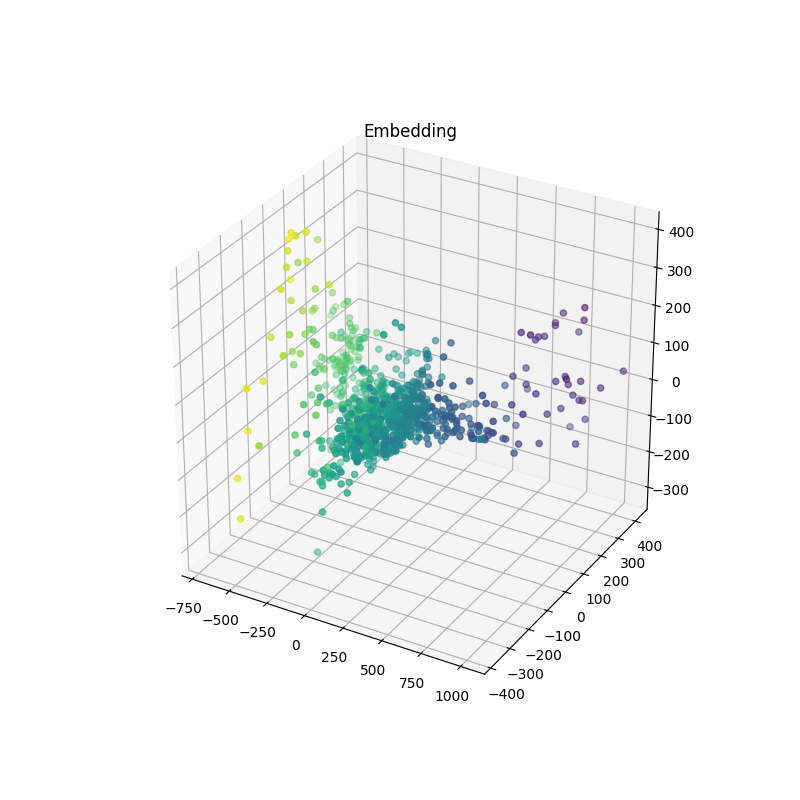
\includegraphics[width=1\textwidth,center]{bilder/Hauptteil/MT_Grapple/EMB_alle/1_Embedding_y.png}
		\caption{V:1 y-Position}
		\label{img:Einbettung1_y}	
	\end{subfigure}
	\centering
	\begin{subfigure}[c]{0.49\textwidth}			
		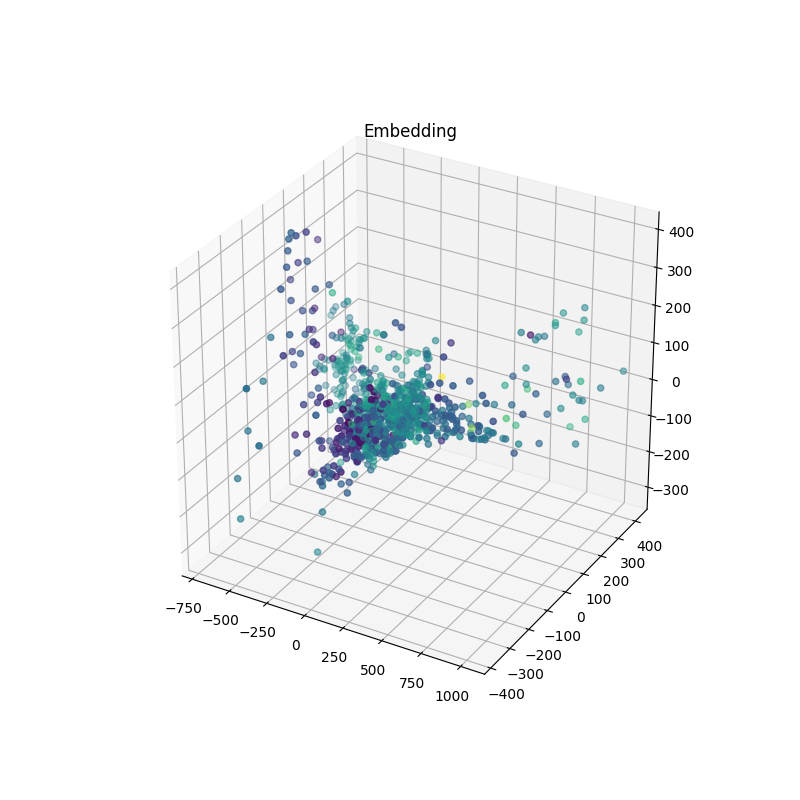
\includegraphics[width=1\textwidth,center]{bilder/Hauptteil/MT_Grapple/EMB_alle/1_Embedding_x.png}
		\caption{V:1 x-Position}
		\label{img:Einbettung1_x}		
	\end{subfigure}
	
	\begin{subfigure}[c]{0.49\textwidth}			
		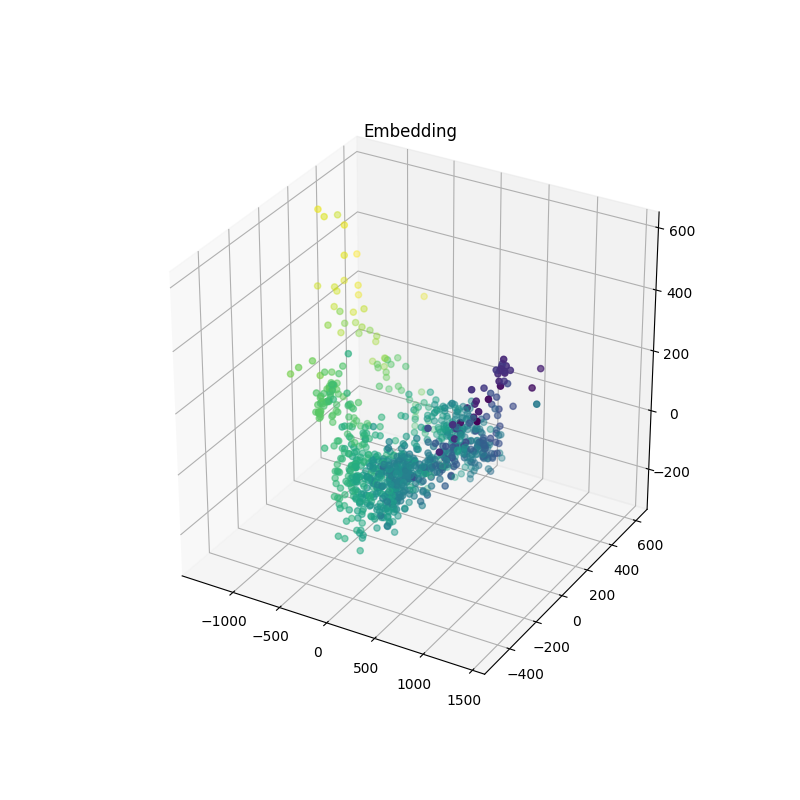
\includegraphics[width=1\textwidth,center]{bilder/Hauptteil/MT_Grapple/EMB_alle/2_Embedding_y.png}
		\caption{V:2 y-Position}
		\label{img:Einbettung2_y}	
	\end{subfigure}
	\centering
	\begin{subfigure}[c]{0.49\textwidth}			
		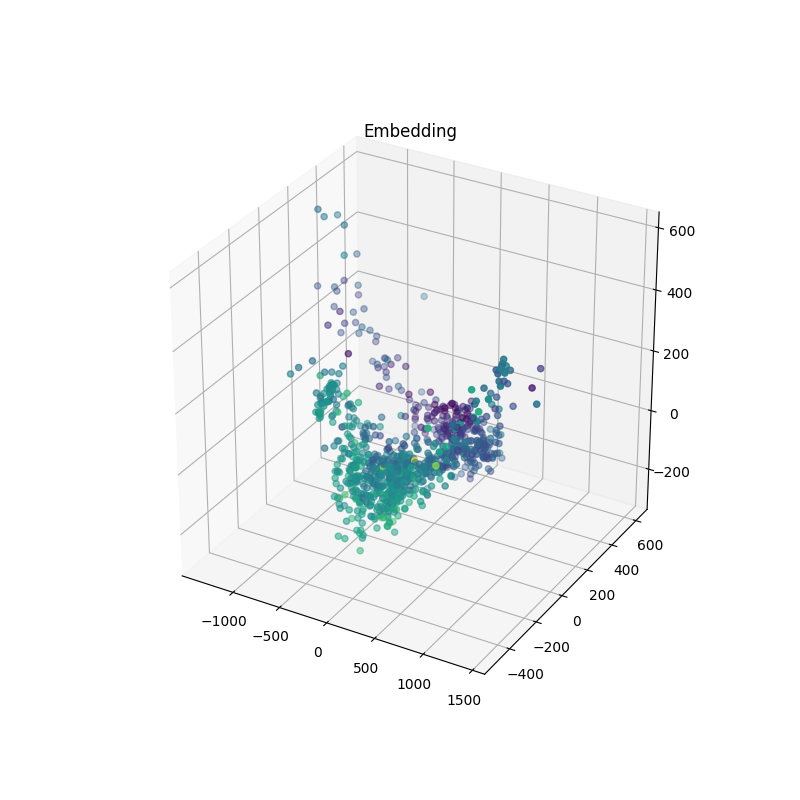
\includegraphics[width=1\textwidth,center]{bilder/Hauptteil/MT_Grapple/EMB_alle/2_Embedding_x.png}
		\caption{V:2 x-Position}
		\label{img:Einbettung2_x}		
	\end{subfigure}
	
	\begin{subfigure}[c]{0.49\textwidth}			
		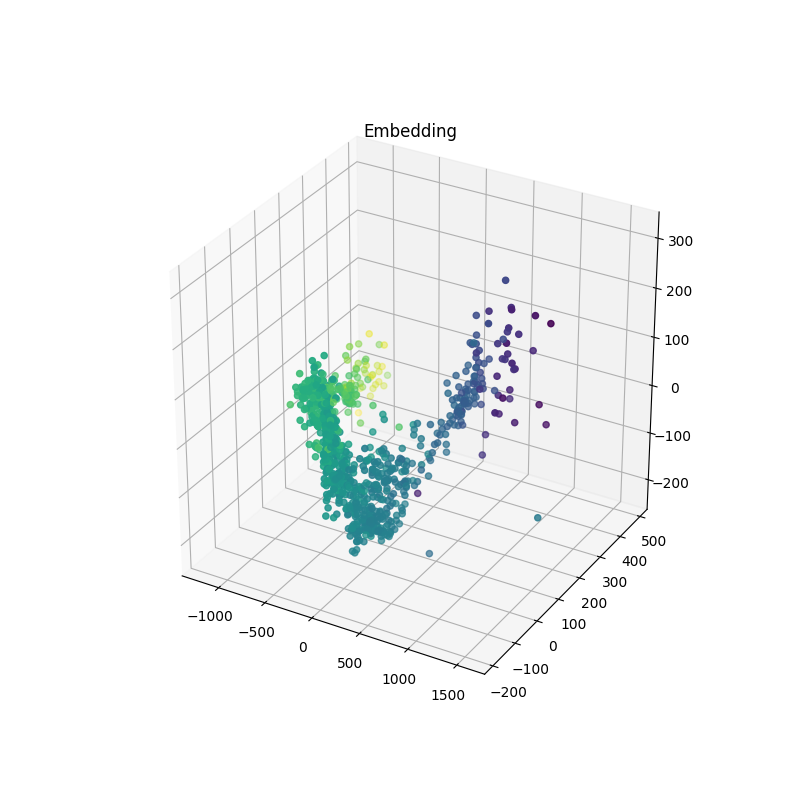
\includegraphics[width=1\textwidth,center]{bilder/Hauptteil/MT_Grapple/EMB_alle/3_Embedding_y.png}
		\caption{V:3 y-Position}
		\label{img:Einbettung3_y}	
	\end{subfigure}
	\centering
	\begin{subfigure}[c]{0.49\textwidth}			
		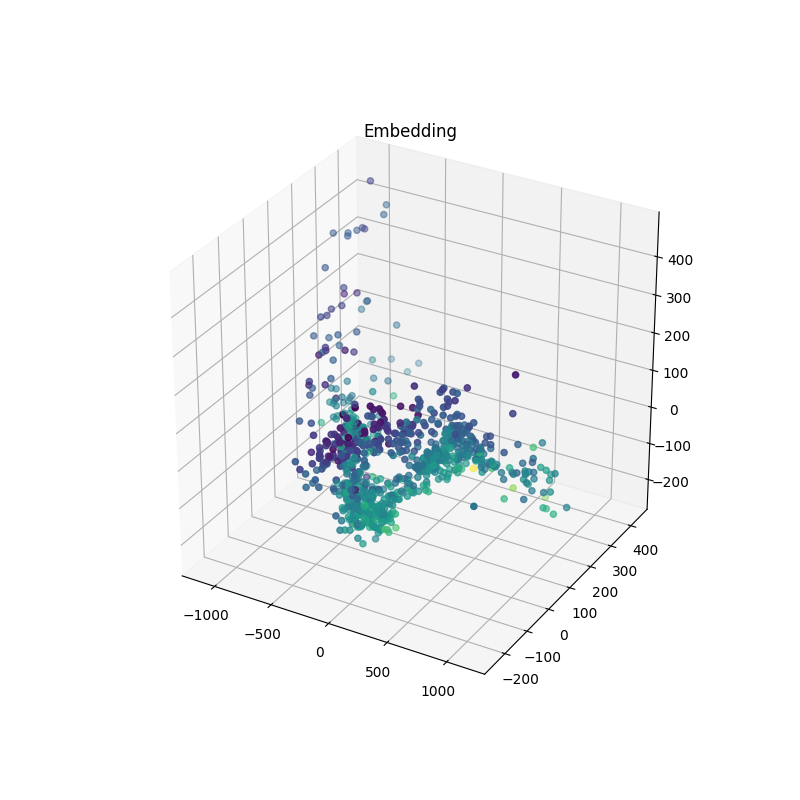
\includegraphics[width=1\textwidth,center]{bilder/Hauptteil/MT_Grapple/EMB_alle/3_Embedding_x.png}
		\caption{V:3 x-Position}
		\label{img:Einbettung3_x}		
	\end{subfigure}
	
	\caption{Einbettungen TFAE-Greifererkennung V:1-3}
	\label{img:Einbettungen1-3}
\end{figure}

	\begin{figure}[h]
		\centering
		\includegraphics[width=0.7\textwidth, center]{bilder/Hauptteil/MT_Grapple/Fehler/schwarzGrappleWrong.png}
		\caption{'Rahmen um Greifer' falsch vorhergesagt}
		\label{img:GrappleFalschVorhergesagt}
	\end{figure}
